\section{Design and Implementation}
\label{sec:design}

\subsection{Design Goals}

With the creation of \houdini, we sought to rectify a critical perceived gap in existing
security testing frameworks. In particular, we noticed that no existing testing framework
satisfied our specific use case: testing the isolation guarantees of a research artifact
in a highly reproducible manner, independent of the underlying container runtime and the
implementation details of the enforcement mechanism. (Refer to \Cref{sec:related} for
a detailed comparison with existing work on container security evaluation.)

In order to achieve the aforementioned result, we designed \houdini with the following
goals in mind:
\begin{dgenum}
  \item \label{dg:repro}\textit{Reproducible Results.} Results of a test should be
  reproducible over time and across various system configurations. Reproducibility is
  a critical property of the scientific method and quintessential to the integrity of
  academic research evaluations. Our hope is that reproducible security evaluations will
  promote the use of \houdini to enable fair and unbiased comparisons of container security
  artifacts based on their security properties.

  \item \label{dg:platform}\textit{Controlled Environment.} \houdini should be capable of
  evaluating a security artifact independently of the underlying platform (e.g\@. the
  container runtime, host operating system, and whatever security measures are in place,
  if any). Platform independence helps to ensure that the focus of a security evaluation
  is on the effectiveness of whatever protections are being tested as opposed to
  differences in the underlying platform (e.g\@. bugs, configuration differences, or
  version specific behaviors).

  \item \label{dg:container}\textit{Container Specificity.} While a number of security
  testing frameworks exist, very few target the container specific use case we want to
  support with \houdini: container security. This motivated us to consider an
  implementation which focuses specifically on the container security use case.

  \item \label{dg:flex}\textit{Test Case Expressiveness.} \houdini test cases (called
  \enquote{tricks}) should be maximally expressive, such that some combination of steps
  can be used to achieve and test any desired result. It should be possible to define
  a new \houdini trick and modify existing tricks without modifying the \houdini
  binary. Moreover, it should be clear from reading a defined trick precisely what steps
  are involved, the consequences of each step passing or failing, and the overall nature
  of the exploit being tested.
\end{dgenum}

We wrote \houdini in just over 3300 lines of Rust code\footnote{Source lines of code,
i.e\@. not counting whitespace, comments, and dependencies.}. Rust offers several
desirable properties for a security benchmarking application like \houdini. First, Rust
has a rich ecosystem of libraries (called \enquote{crates}) that enable us to easily work
with external APIs such as the Docker daemon. Moreover, Rust has excellent support for
serializing and deserializing YAML and JSON to and from Rust enums and data structures using
powerful macros exposed by the \texttt{serde} crate. Finally, Rust's \texttt{tokio} crate
provides a powerful asynchronous framework that enables us to easily parallelize and
synchronize \houdini tricks and their steps.

\todo{talk about security and how we shouldn't need to worry about the tricks being used
maliciously (we're testing armour and brining our own weapons and test range, we're not
really worried terrorists coming in and blowing us up)}

\subsection{Houdini Tricks}

Exploits that \houdini can test are broken up into individual files called
\textit{tricks} (\Cref{dg:flex}). Each \houdini trick is written in YAML and consists of a metadata section
followed by one or more \textit{steps}. \houdini comes with a stock set of tricks (c.f\@.
\Cref{sec:testing-confinement}), tested in continuous integration to ensure they always
work by default under vulnerable configurations.

While these default tricks can provide decent exploit coverage for initial tests, it is
also possible for the user to write their own tricks by defining their own YAML files
following the expected format. This modular design enables \houdini to test essentially
any container escape while providing the ability for the user to modify existing tricks
should the need arise (e.g\@. to test a specific aspect of a defense mechanism in a more
targeted fashion).

\Cref{lst:mounted-docker-socket} provides a simple example of a \houdini trick that tests
whether a mounted Docker socket in a container can be used to communicate with the Docker
daemon running on the host. Steps in a \houdini trick consist of an ordered list of
parameterized, well-defined actions. In our current implementation, there are six distinct
types of step:

\begin{itemize}
  \item \texttt{VersionCheck} enforces a version check on the host operating system version,
  docker daemon version, and container runtime version (e.g\@. \texttt{runc}). This helps
  to verify that a trick is indeed running under an expected configuration where it
  would ordinarily succeed without any additional protections in place.

  \item \texttt{SpawnContainer}

  \item \texttt{KillContainer}

  \item \texttt{Host}

  \item \texttt{Container}

  \item \texttt{Wait}
\end{itemize}

\begin{listing}
  \caption{A YAML definition of a Houdini trick with three steps. The first step spawns
  a container from the \enquote{bash} Docker image, downloading it if necessary. As part
  of the exploit setup, we mount \texttt{/var/run/docker.sock} from the host into the
  container. The second step installs curl into the bash container. Finally, the third
  step attempts to abuse the mounted Docker socket to make API requests to Docker. Note the
  status codes on success and failure for each step in the Trick.}
  \label{lst:mounted-docker-socket}
  \begin{minted}[frame=lines,framesep=2mm]{yaml}
  name: mounted-docker-socket
  steps:
    - spawnContainer:
        name: bash
        image: bash
        cmd: sleep infinity
        volumes:
        - "/var/run/docker.sock:/docker.sock"
        failure: setupFailure
    - container:
        name: bash
        script:
        - command: apk
          args:
          - add
          - curl
        failure: setupFailure
    - container:
        name: bash
        script:
        - command: curl
          args:
          - "--unix-socket"
          - "/docker.sock"
          - "http://localhost/_ping"
        failure: exploitFailure
        success: exploitSuccess
  \end{minted}
\end{listing}

\subsection{Reproducible Tricks}

\todo{WILLIAM: Houdini design and implementation details here.}


\begin{figure}
  \label{fig:state-machine}
  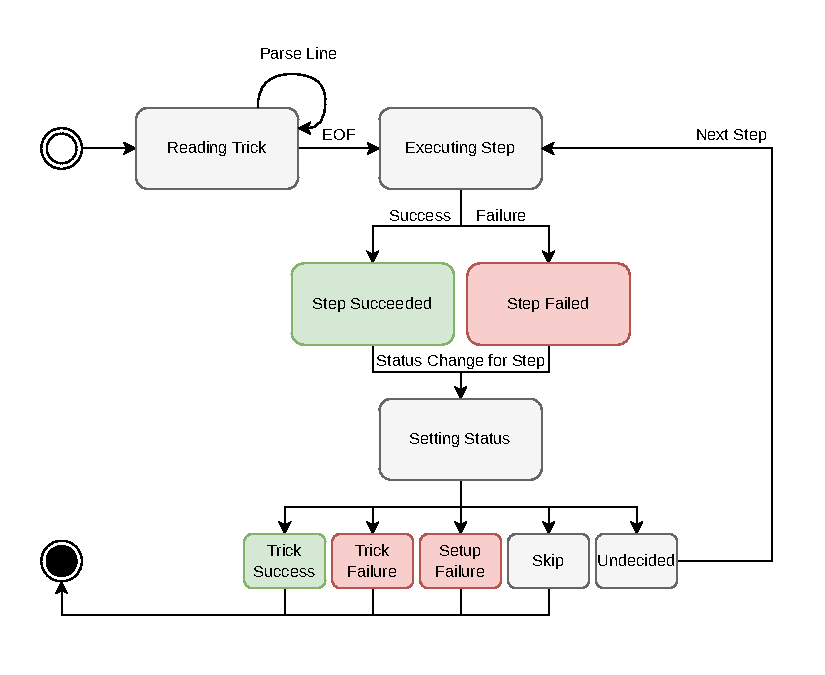
\includegraphics[width=1\linewidth]{figs/houdini-state-machine.pdf}
  \caption{A state machine diagram of Houdini running a Trick. Note that aside from the
  \enquote{Undecided} status, all other statuses are considered final. That is, a step
  reporting such a status terminates execution of the Trick.}
\end{figure}

\todo{WILLIAM: Introduce the architecture diagram below somehow (what is the best way to do this?)}

\begin{itemize}
\item security problems arise from vuln in specific components
\item if we're going to be testing, we need to have an idea of what components we're testing
\item ideal coverage will touch everything
\item some components are targeted more frequently than others in attacks commonly used in practice
\end{itemize}

\begin{figure}
  \label{fig:architecture}
  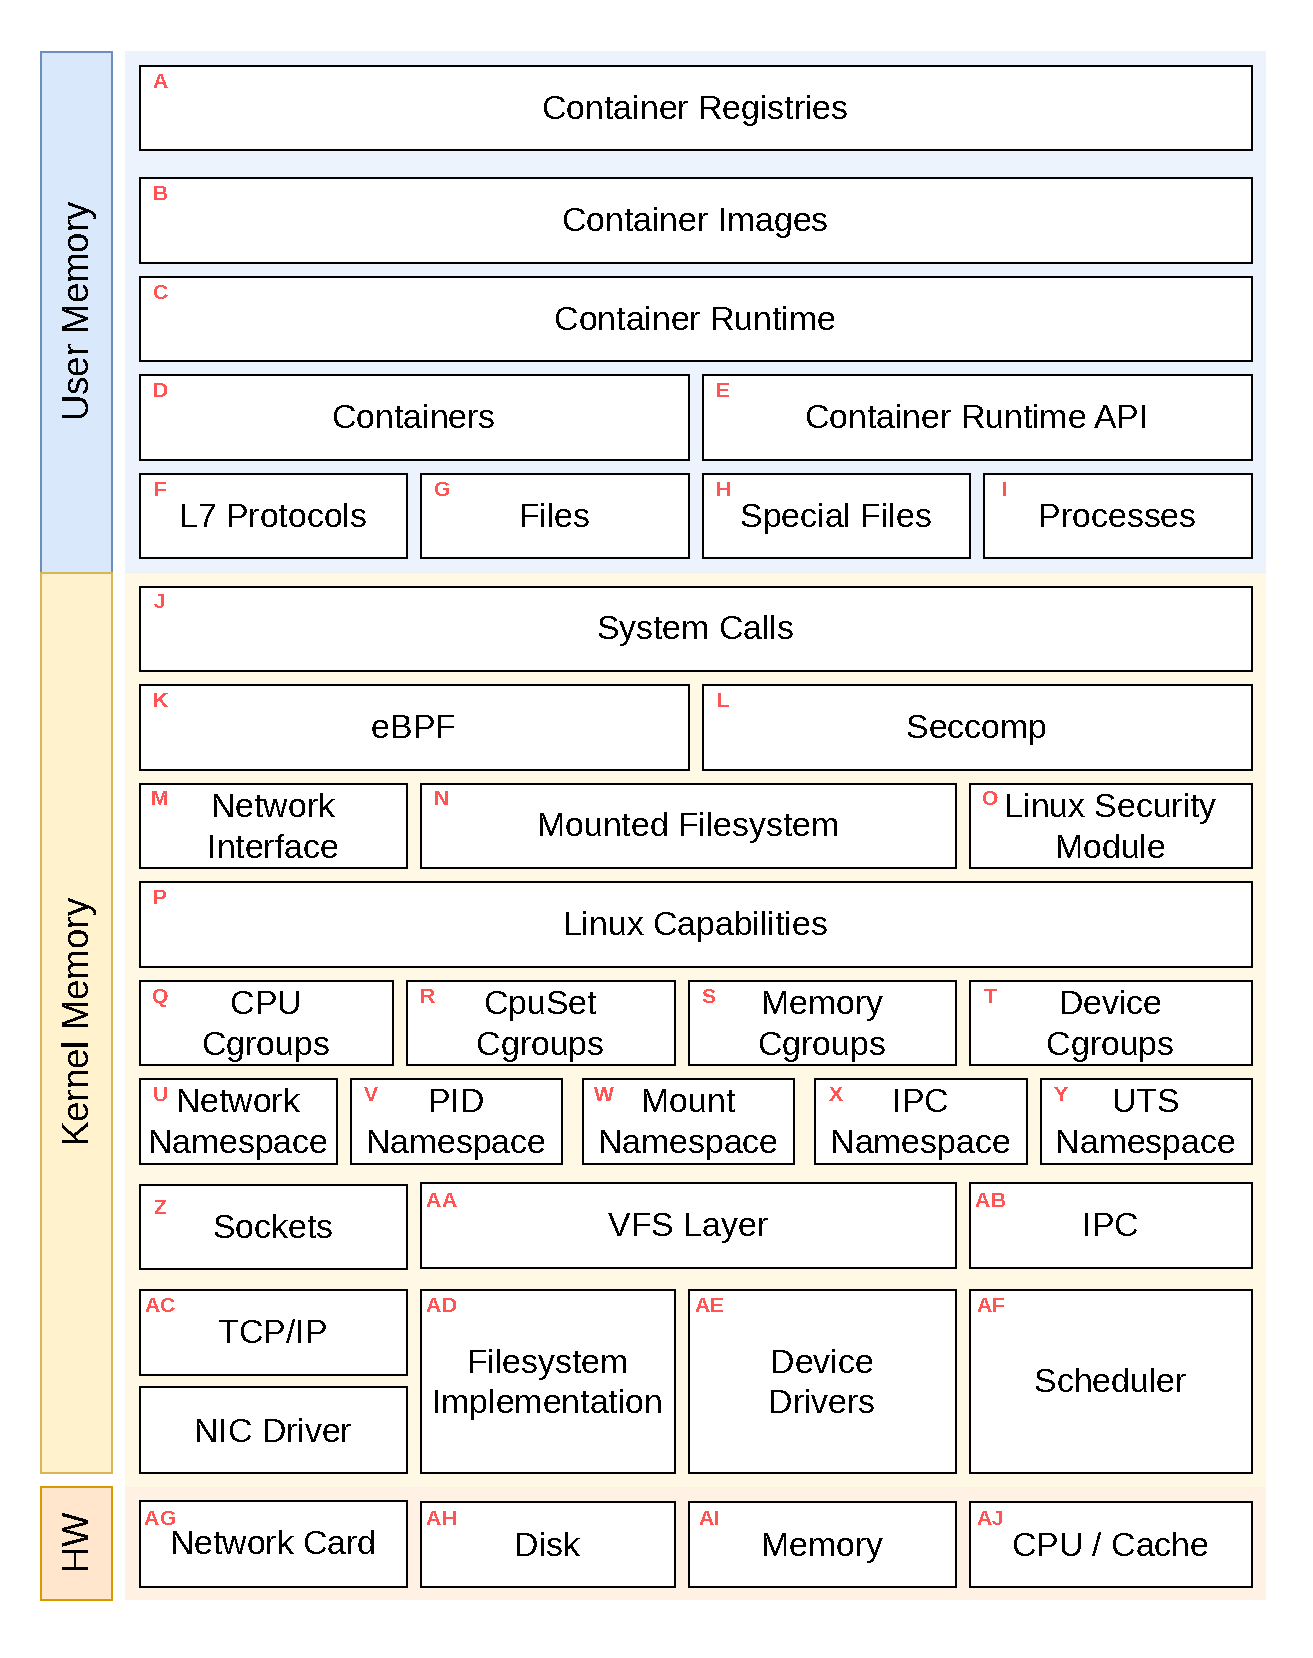
\includegraphics[width=1\linewidth]{figs/exploit-coverage.pdf}
  \caption{An architectural diagram of a container deployment environment depicting the
  attack surface created by its various components. Components are organized
  hierarchically with lower level subsystems toward the bottom, including data structures
  and abstractions that reside in kernel memory and the hardware itself.}
\end{figure}
